\documentclass[oneside,draft]{book}

\usepackage[utf8]{inputenc}
\usepackage[spanish]{babel}

\usepackage{amsmath,amssymb}

\usepackage[colorlinks,final]{hyperref}

\hypersetup{
    colorlinks,
    linkcolor={red!60!black},
    citecolor={blue!60!black},
    urlcolor={blue!80!black}
}

\usepackage{amsthm}
\newtheorem{proposicion}{Proposición}[chapter]
\newtheorem{corolario}[proposicion]{Corolario}
\newtheorem{lema}[proposicion]{Lema}
\newtheorem{teorema}[proposicion]{Teorema}
\newtheorem{conjetura}[proposicion]{Conjetura}

\theoremstyle{definition}
\newtheorem{algoritmo}[proposicion]{Algoritmo}
\newtheorem{comentario}[proposicion]{Comentario}
\newtheorem{definicion}[proposicion]{Definición}
\newtheorem{ejemplo}[proposicion]{Ejemplo}

\newtheorem{ejercicio}{Ejercicio}[chapter]

\newcommand{\NN}{\mathbb{N}}
\newcommand{\ZZ}{\mathbb{Z}}
\newcommand{\QQ}{\mathbb{Q}}
\newcommand{\RR}{\mathbb{R}}
\newcommand{\CC}{\mathbb{C}}

\renewcommand{\Re}{\operatorname{Re}}

\DeclareMathOperator{\mcd}{mcd}
\DeclareMathOperator{\mcm}{mcm}
\DeclareMathOperator{\ord}{ord}
\DeclareMathOperator{\sgn}{sgn}
\DeclareMathOperator{\li}{li}

\newcommand{\legendre}[2]{\left(\frac{#1}{#2}\right)}

\usepackage{framed}

\usepackage[final]{graphicx}

\usepackage[dvipsnames]{xcolor}
\definecolor{shadecolor}{rgb}{0.79,0.78,0.65}
\usepackage{colortbl}

\newcommand\hl[1]{\fboxsep=0pt\colorbox{shadecolor}{$\displaystyle#1$}}

\usepackage{tikz-cd}
\usetikzlibrary{babel}

\newcommand*\circled[1]{\tikz[baseline=(char.base)]{\node[shape=circle,draw,inner sep=2pt] (char) {#1};}}

\usepackage{cancel}

\renewcommand*{\thefootnote}{(\arabic{footnote})}

\usepackage[numbers]{natbib}

\newcommand\oeis[1]{[\href{https://oeis.org/#1}{#1}]}

\usepackage{array}
\newcolumntype{x}[1]{>{\centering\hspace{0pt}}p{#1}}
\usepackage{diagbox}

\def\mystrut(#1,#2){\vrule height #1 depth #2 width 0pt}

\newcolumntype{f}[1]{%
>{\mystrut(3ex,2ex)\centering}%
p{#1}%
<{}}

\begin{document}

%% \tableofcontents

%%%%%%%%%%%%%%%%%%%%%%%%%%%%%%%%%%%%%%%%%%%%%%%%%%%%%%%%%%%%%%%%%%%%%%%%%%%%%%%%

\iffalse
\input{introduccion.tex}
\input{preliminares.tex}
\fi

%% \part{Aritmética de los números enteros}
\ifdefined\handout
  \documentclass[handout]{beamer}
\else
  \documentclass{beamer}
\fi

\usetheme{boxes}
\usecolortheme{structure}

\setbeamertemplate{footline}[frame number]

\ifdefined\handout
\definecolor{beamer@structure@color}{rgb}{0,0,0}
\setbeamertemplate{navigation symbols}{}
\setbeamercolor{normal text}{fg=black,bg=white}
\setbeamertemplate{frametitle}{\vskip 15pt\color{black}
\def\myhrulefill{\leavevmode\leaders\hrule height 1pt\hfill\kern 0pt}
\headingfont\insertframetitle\par\vskip-8pt\myhrulefill}
\else
\definecolor{beamer@structure@color}{rgb}{1,1,1}
\setbeamertemplate{navigation symbols}{}
\setbeamercolor{normal text}{fg=white,bg=black}
\setbeamertemplate{frametitle}{\vskip 15pt\color{white}
\def\myhrulefill{\leavevmode\leaders\hrule height 1pt\hfill\kern 0pt}
\headingfont\insertframetitle\par\vskip-8pt\myhrulefill}
\fi

\usepackage{amsmath,amssymb}

\newcommand{\NN}{\mathbb{N}}
\newcommand{\ZZ}{\mathbb{Z}}

\DeclareMathOperator{\mcd}{mcd}
\DeclareMathOperator{\mcm}{mcm}

\usepackage[spanish]{babel}

\usepackage{tikz-cd}
\usetikzlibrary{babel}
\usetikzlibrary{calc}

\usepackage{framed}

\newcommand{\dfn}{\mathrel{\mathop:}=}
\newcommand{\rdfn}{=\mathrel{\mathop:}}

\usepackage{mathspec}
\setsansfont[BoldFont={IBM Plex Sans Bold}, ItalicFont={IBM Plex Sans Italic}]{IBM Plex Sans}
\setmonofont[BoldFont={IBM Plex Mono Bold}, ItalicFont={IBM Plex Mono Italic}]{IBM Plex Mono}
\setmathrm[BoldFont={IBM Plex Sans Bold}, ItalicFont={IBM Plex Sans Italic}]{IBM Plex Sans}
\newfontfamily\headingfont[]{IBM Plex Sans Bold}

\setbeamercovered{transparent=10}


\begin{document}

\begin{frame}[plain,noframenumbering]
  \textbf{INTRODUCCIÓN A LA TEORÍA DE NÚMEROS}

  Alexey Beshenov $\mid$ \texttt{cadadr.org}

  \vfill

  \begin{center}\huge\headingfont
    DIVISIBILIDAD DE LOS NÚMEROS ENTEROS
  \end{center}

  \vfill
\end{frame}

\begin{frame}
  \frametitle{NÚMEROS NATURALES Y ENTEROS}

  \begin{itemize}
  \item<2-> Los números \textbf{naturales}:
    $\NN = \{ 0, 1, 2, 3, \ldots \}$.

  \item<3-> Los números \textbf{enteros}:
    $\ZZ = \{ \ldots, -3, -2, -1, 0, +1, +2, +3, \ldots \}$.

  \item<4-> Operaciones aritméticas:

    «$+$» (\textbf{suma}),
    «$\cdot$» (\textbf{producto}),
    «$-$» (\textbf{resta}, para $\ZZ$).

  \item<5-> Axiomatización: interesante, pero nos llevaría lejos\dots

  \item<6-> La \textbf{teoría de números} estudia las propiedades aritméticas de
    los números enteros\onslide<7->{\dots{} y otros objetos mucho más
      sofisticados que ayudan a entender los enteros.}

  \item<8-> Hoy: la relación de \textbf{divisibilidad}.
  \end{itemize}
\end{frame}

\begin{frame}
  \frametitle{DEFINICIÓN}

  \begin{itemize}
  \item<2-> Sean $a, b \in \ZZ$ enteros.

  \item<3-> «$b \mid a$» si existe un entero $c$ tal que $a = bc$.

  \item<4-> «$a$ es \textbf{divisible} por $b$»,

    \onslide<5->{«$b$ \textbf{divide} al número $a$»,}

    \onslide<6->{«$b$ es un \textbf{divisor} de $a$».}

  \item<7-> Si $a$ no es divisible por $b$, se escribe «$b\nmid a$».
  \end{itemize}
\end{frame}

\begin{frame}
  \frametitle{EJEMPLO: ¿DOCENA O DECENA?}

  \begin{minipage}[t][0.6\textheight]{0.6\textwidth}
    \vspace{0pt}
    \begin{itemize}
    \item<2-> ¿Por qué los huevos suelen venderse por docena ($12$) y no por
      decena ($10$)?

    \item<3-> Los divisores (positivos) de $12$ son $1$, $2$, $3$, $4$, $6$,
      $12$.

    \item<4-> Los divisores (positivos) de $10$ son $1$, $2$, $5$, $10$.

    \item<5-> ¡Más práctico dividir $12$!
    \end{itemize}
  \end{minipage}
  \begin{minipage}[t]{0.35\textwidth}
    \vspace{0pt}\flushright
    \onslide<2->{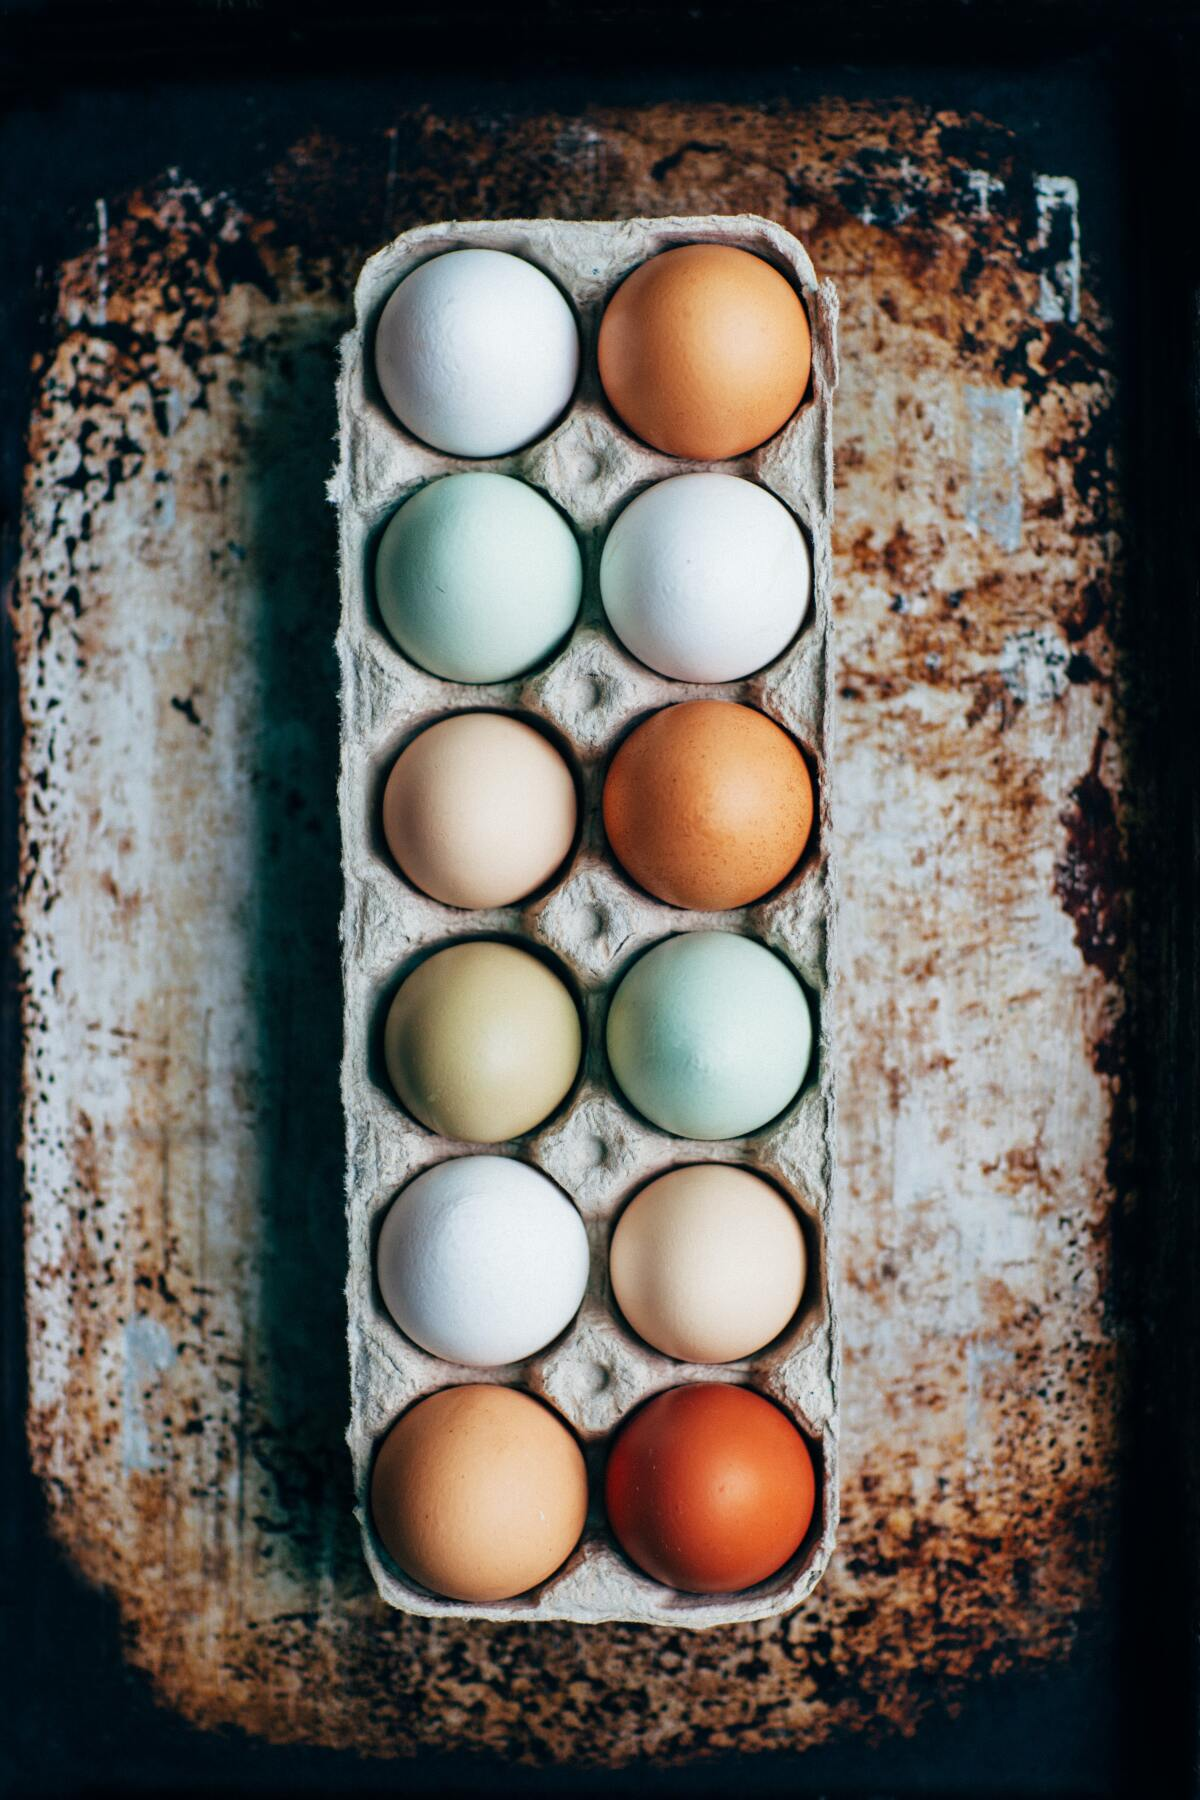
\includegraphics[width=.9\textwidth]{eggs.jpg}}
  \end{minipage}
\end{frame}

\begin{frame}
  \frametitle{OTRAS COSAS QUE SE VENDEN POR DOCENA}

  \begin{center}
    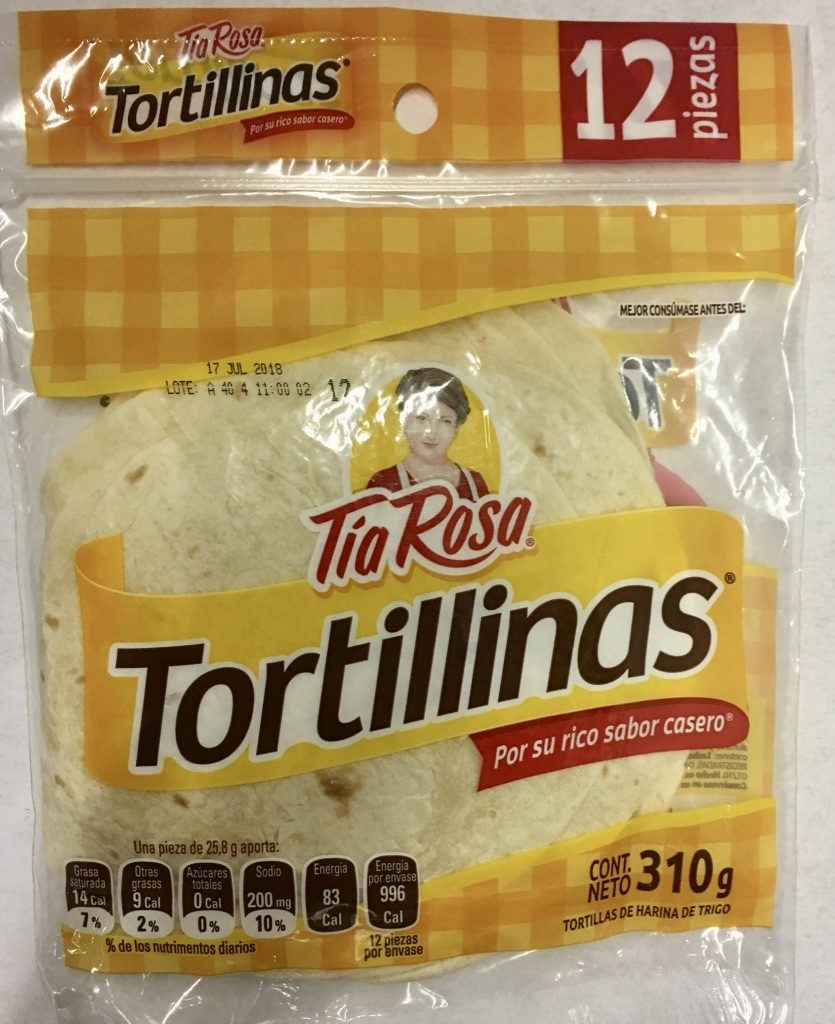
\includegraphics[width=0.4\textwidth]{tia-rosa.jpg}
  \end{center}
\end{frame}

\begin{frame}
  \frametitle{EJEMPLO: 60 MINUTOS Y 60 SEGUNDOS}

  \begin{minipage}[t][0.6\textheight]{0.6\textwidth}
    \vspace{0pt}
    \begin{itemize}
    \item<2-> Los divisores (positivos) de $60$ son
      $1$, $2$, $3$, $4$, $5$, $6$, $10$, $12$, $15$, $20$, $30$, $60$.

    \item<3-> Muy cómodo dividir una hora en $60$ minutos y un minuto en $60$
      segundos.

    \item<4-> $100$ tiene menos divisores:

      $1$, $2$, $4$, $5$, $10$, $20$, $25$, $50$, $100$.

    \item<5-> Influencia muy antigua babilónica (c. 2000 a.C.):

      sistema de numeración \textbf{sexagesimal} (base $60$).
    \end{itemize}
  \end{minipage}
  \begin{minipage}[t]{0.35\textwidth}
    \vspace{0pt}\flushright
    \onslide<2->{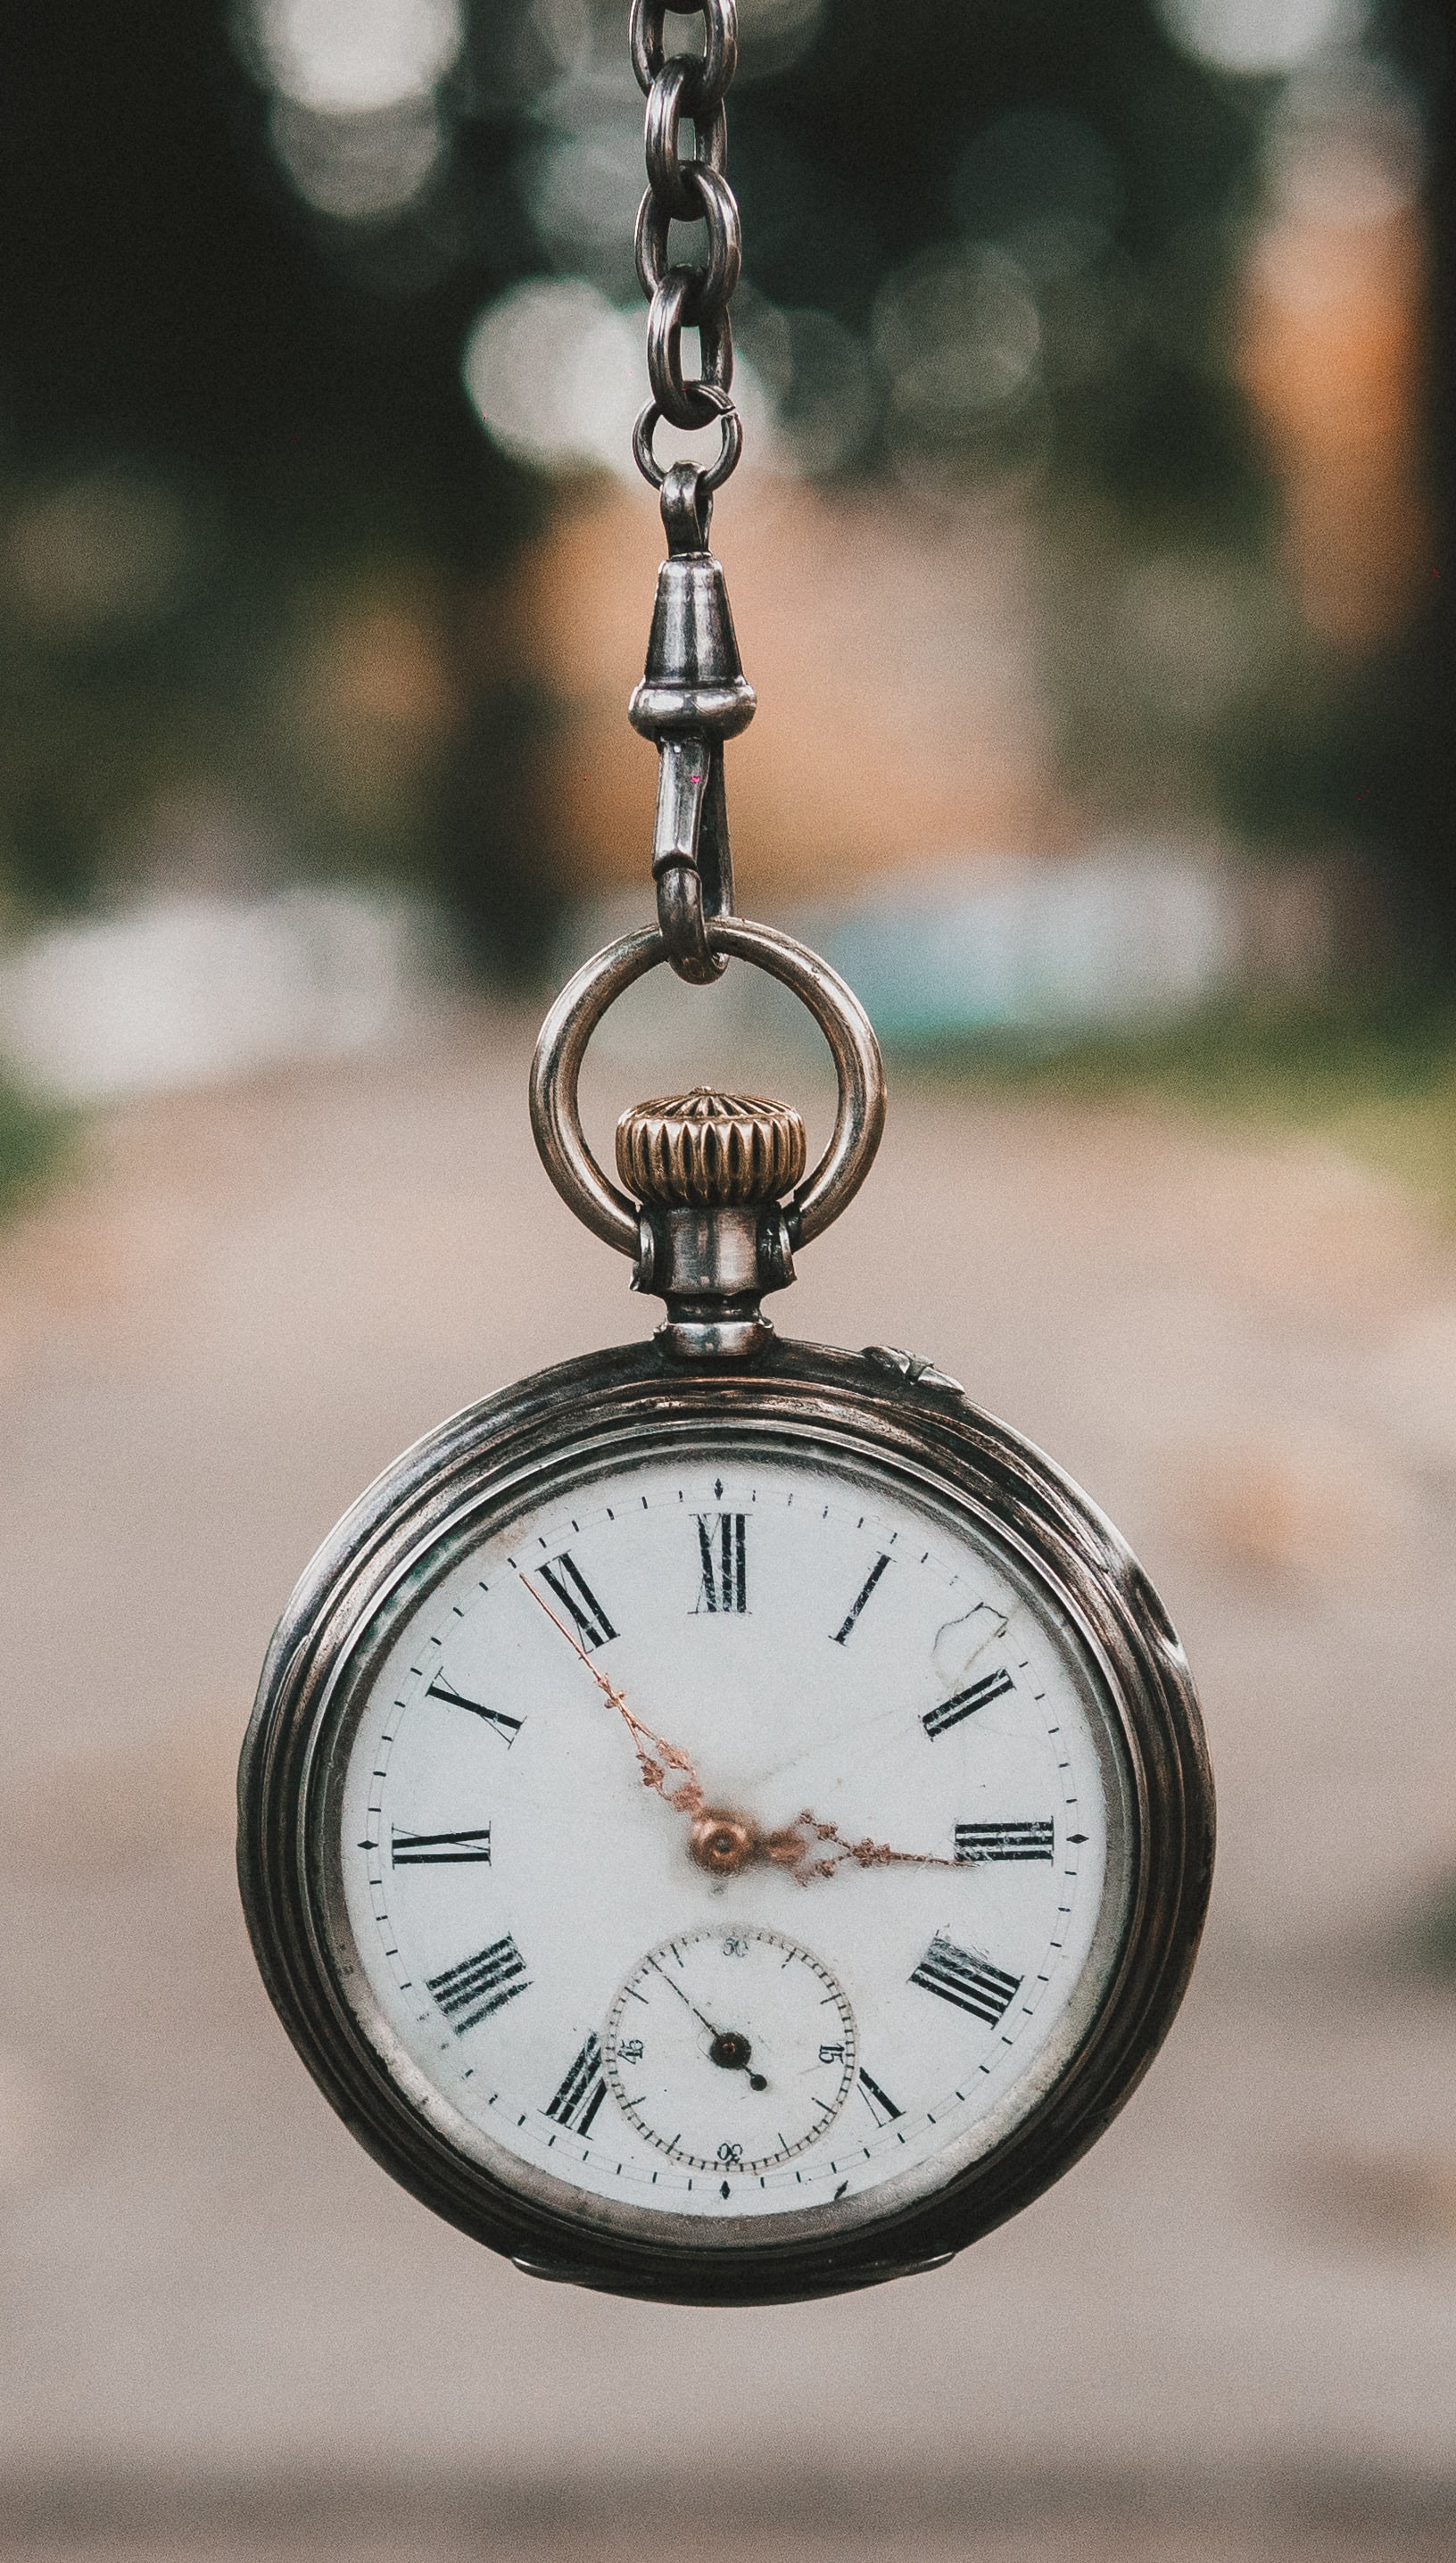
\includegraphics[width=.9\textwidth]{clock.jpg}}
  \end{minipage}
\end{frame}

\begin{frame}
  \frametitle{NUMERACIÓN BABILÓNICA}

  \begin{center}
    
\includegraphics[width=\textwidth]{babylonian.pdf}
  \end{center}
\end{frame}

\begin{frame}
  \frametitle{EJEMPLO: 360 GRADOS}

  \begin{minipage}[t][0.8\textheight]{0.6\textwidth}
    \vspace{0pt}
    \begin{itemize}
    \item<2-> La división del círculo en $360$ \textbf{grados} viene de la misma
      influencia babilónica.

    \item<3-> $360 = 6 \cdot 60$.

    \item<4-> Divisores (positivos) de $360$:

      $1$, $2$, $3$, $4$, $5$, $6$, $8$, $9$, $10$, $12$, $15$, $18$, $20$,
      $24$, $30$, $36$, $40$, $45$, $60$, $72$, $90$, $120$, $180$, $360$.

    \item<5-> Convención totalmente arbitraria, pero práctica.

    \item<6-> Los matemáticos de hoy dividen el círculo en 2π \textbf{radianes}.
    \end{itemize}
  \end{minipage}
  \begin{minipage}[t]{0.35\textwidth}
    \vspace{0pt}\flushright
    \onslide<2->{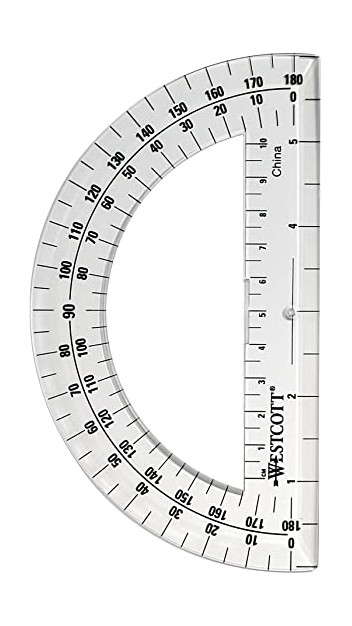
\includegraphics[width=.9\textwidth]{protractor.jpg}}
  \end{minipage}
\end{frame}

\begin{frame}
  \frametitle{EJEMPLO: COORDENADAS GEOGRÁFICAS}

  \begin{minipage}[t][0.8\textheight]{0.6\textwidth}
    \vspace{0pt}
    \begin{itemize}
    \item<2-> Hiparco de Nicea \\
      (c. 190 a.C. -- 120 a.C.):

      la división del día en $24$ horas,

      las \textbf{coordenadas geográficas}.

    \item<3-> Influencia babilónica.

    \item<4-> Latitud $0$--$180^\circ$ norte / sur.

    \item<5-> Longitud $0$--$180^\circ$ este / oeste.

    \item<6-> $60$ minutos (${}'$) en cada grado.

    \item<7-> $60$ segundos (${}''$) en cada minuto.

    \item<8-> Ejemplo: la Ciudad de México,

      $19^\circ$ $25'$ $10''$ N,
      $99^\circ$ $8'$ $44''$ O.
    \end{itemize}
  \end{minipage}
  \begin{minipage}[t]{0.35\textwidth}
    \vspace{0pt}\flushright
    \onslide<2->{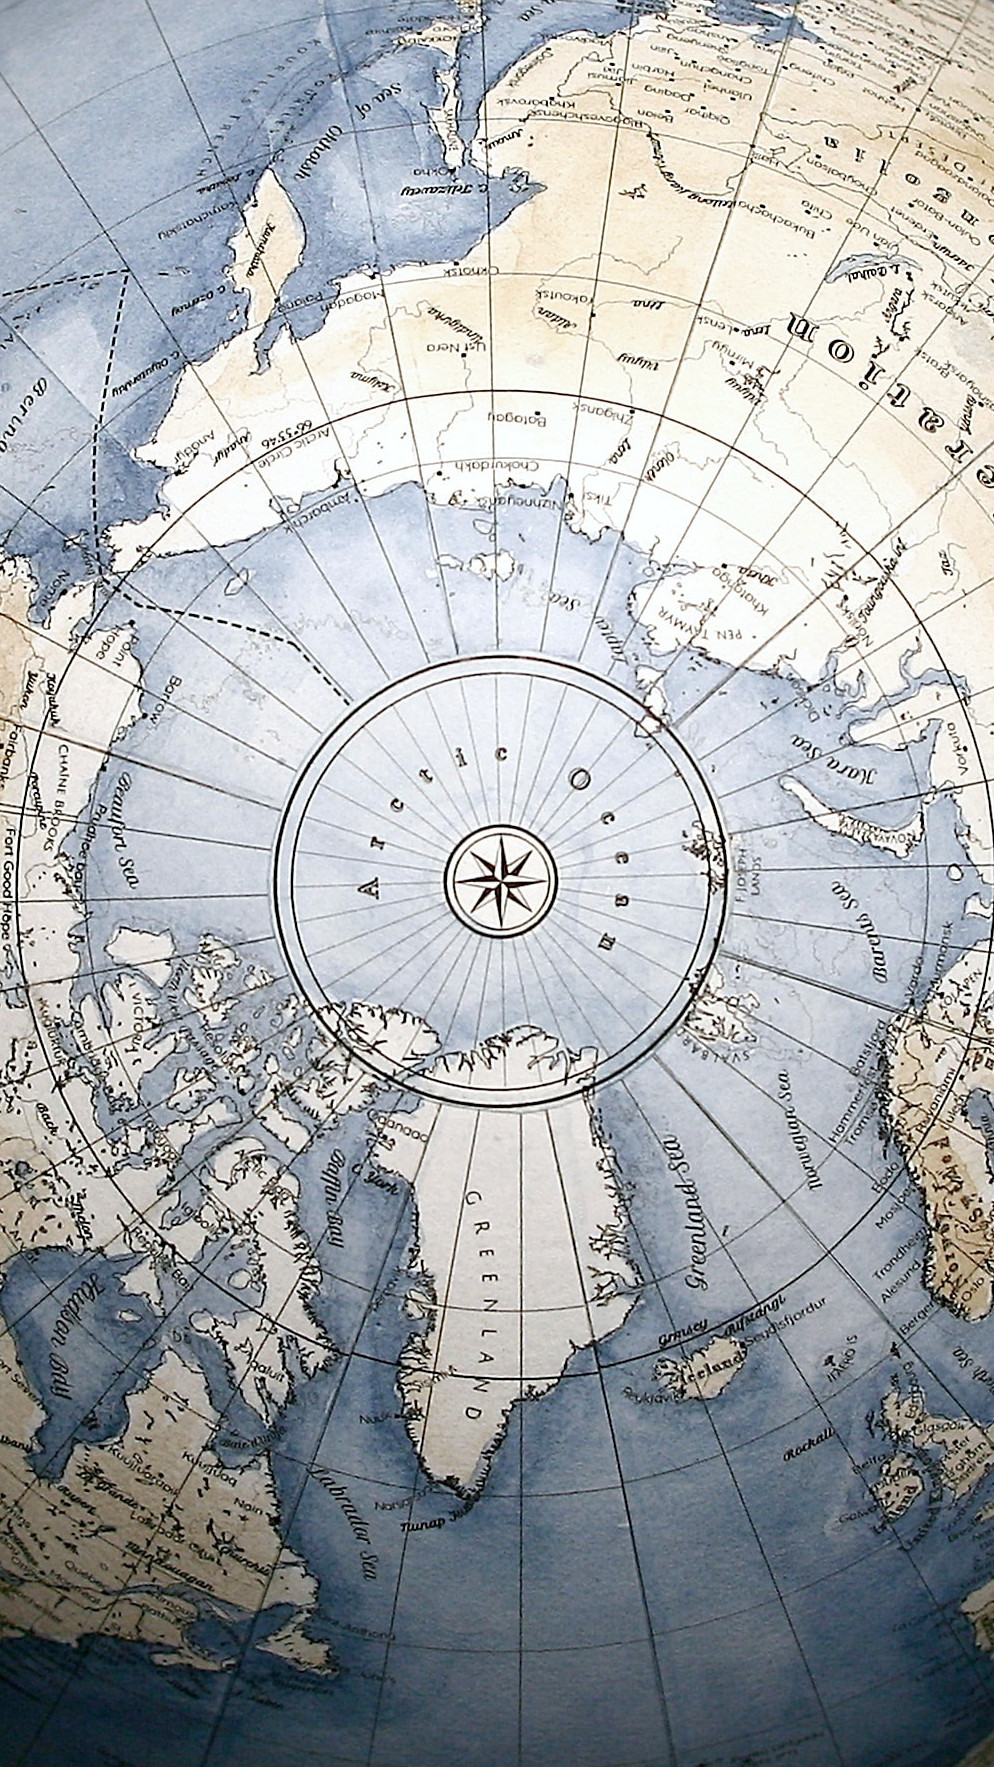
\includegraphics[width=.9\textwidth]{globe.jpg}}
  \end{minipage}
\end{frame}

\begin{frame}
  \frametitle{NÚMEROS PRIMOS}

  \begin{itemize}
  \item<2-> $7$ tiene como sus divisores $\pm 1$ y $\pm 7$.

  \item<3-> $23$ tiene como sus divisores $\pm 1$ y $\pm 23$.

  \item<4-> Son \textbf{números primos}.

  \item<5-> $360$ tiene muchos divisores, pero

    $359$ es divisible solo por $\pm 1$ y $\pm 359$; es primo.

  \item<6-> Los primeros primos son

    $2$, $3$, $5$, $7$, $11$, $13$, $17$, $19$, $23$, $29$, $31$, $37$, $41$,
    $43$, $47$, $53$, $59$, $61$, $67$, $71$, $73$, $79$, $83$, $89$, $97$,
    $101$, $\ldots$

  \item<7-> El número $\pm 1$ no se considera como primo.
  \end{itemize}
\end{frame}

\begin{frame}
  \frametitle{PROPIEDADES DE DIVISIBILIDAD}

  \begin{itemize}
  \item<2-> Si $b \mid a$, entonces $|b| \le |a|$.

    \onslide<3->{\emph{Demostración}: si $a = bc$, entonces $|a| = |b|\cdot |c|$.}

  \item<4-> \textbf{Corolario}: si $b \mid a$ y $a \mid b$, entonces
    $a = \pm b$.

    \onslide<5->{(Relación \textbf{antisimétrica}, salvo signo.)}
  \end{itemize}
\end{frame}

\begin{frame}
  \frametitle{PROPIEDADES DE DIVISIBILIDAD (CONT.)}

  \begin{enumerate}
  \item<2->[1)] $1\mid a$, $a \mid a$, $a \mid 0$ para cualquier $a$,

  \item<3->[2)] $a\mid 1$ si y solamente si $a = \pm 1$,

  \item<4->[3)] $0\mid a$ si y solamente si $a = 0$,

  \item<5->[4)] si $c \mid a$ y $c \mid b$, entonces $c \mid (a \pm b)$,

  \item<6->[5)] \textbf{transitividad}:

    si $c \mid b$ y $b \mid a$, entonces $c \mid a$,

  \item<7->[6)] \textbf{cancelación}:

    si $c \ne 0$, entonces
    $ac \mid bc$ implica $a\mid b$,

  \item<8->[7)] $b \mid a$ si y solamente si $-b \mid a$.
  \end{enumerate}

  \onslide<9->{\emph{Demostración}. Ejercicio (!)}
\end{frame}

\begin{frame}
  \frametitle{ORDEN PARCIAL SOBRE LOS NATURALES}

  \[ \begin{tikzpicture}[font=\small,x=1.75em, y=1.5em, every node/.style={inner sep=2pt,outer sep=0pt}]
      \draw (0,0) node (n1) {$1$};
      \draw (-1,2) node[circle, draw=white] (n2) {$2$};
      \draw (0,3) node[circle, draw=white] (n3) {$3$};
      \draw (-2,4) node (n4) {$4$};
      \draw (+2,5) node[circle, draw=white] (n5) {$5$};
      \draw (-1,6) node (n6) {$6$};
      \draw (+6,7) node[circle, draw=white] (n7) {$7$};
      \draw (-4,8) node (n8) {$8$};
      \draw (+2,9) node (n9) {$9$};
      \draw (0,10) node (n10) {$10$};
      \draw (+7,11) node[circle, draw=white] (n11) {$11$};
      \draw (-2,12) node (n12) {$12$};

      \draw (n1) -- (n2);
      \draw (n1) -- (n3);
      \draw (n1) -- (n5);
      \draw (n1) -- (n7);
      \draw (n1) -- (n11);

      \draw (n2) -- (n4);
      \draw (n2) -- (n6);
      \draw (n2) -- (n10);

      \draw (n3) -- (n6);
      \draw (n3) -- (n9);

      \draw (n4) -- (n8);
      \draw (n4) -- (n12);

      \draw (n5) -- (n10);

      \draw (n6) -- (n12);

      \draw (n1) -- ($(n1)+(-0.25,1)$);
      \draw (n2) -- ($(n2)+(0,1)$);
      \draw (n3) -- ($(n3)+(0,1)$);
      \draw (n4) -- ($(n4)+(-0.25,1)$);
      \draw (n5) -- ($(n5)+(0,1)$);
      \draw (n6) -- ($(n6)+(0,1)$);
      \draw (n7) -- ($(n7)+(0,1)$);
      \draw (n8) -- ($(n8)+(0,1)$);
      \draw (n9) -- ($(n9)+(0,1)$);
      \draw (n10) -- ($(n10)+(0,1)$);
      \draw (n11) -- ($(n11)+(0,1.5)$);
      \draw (n12) -- ($(n12)+(0,1)$);
    \end{tikzpicture} \]
  \end{frame}

  \begin{frame}
    \frametitle{A CONTINUACIÓN}

    \begin{itemize}
    \item<2-> \textbf{División con residuo} (= \textbf{división euclidiana}).

    \item<3-> Ejemplo: $3\nmid 20$, pero

      \[ \frac{20}{3} = 6\,\frac{2}{3}
        \iff
        20 = 6\cdot 3 + 2. \]

      $2$ es el \textbf{residuo} de división.

    \item<4-> \textbf{Numeración en la base $b$}.

    \item<5-> Ejemplo: $20 = 2^4 + 2^2$, así que

      $20 = \text{\texttt{10100}}$ en la base $2$.
    \end{itemize}
  \end{frame}

\begin{frame}[plain,noframenumbering]

  \vfill

  \begin{center}\huge\headingfont
    ¡GRACIAS POR SU ATENCIÓN!
  \end{center}

  \vfill
\end{frame}
\end{document}

% \input{numeros-primos.tex}
% \input{mcd-y-mcm.tex}
% \ifdefined\handout
  \documentclass[handout]{beamer}
\else
  \documentclass{beamer}
\fi

\usetheme{boxes}
\usecolortheme{structure}

\setbeamertemplate{footline}[frame number]

\ifdefined\handout
\definecolor{beamer@structure@color}{rgb}{0,0,0}
\setbeamertemplate{navigation symbols}{}
\setbeamercolor{normal text}{fg=black,bg=white}
\setbeamertemplate{frametitle}{\vskip 15pt\color{black}
\def\myhrulefill{\leavevmode\leaders\hrule height 1pt\hfill\kern 0pt}
\headingfont\insertframetitle\par\vskip-8pt\myhrulefill}
\else
\definecolor{beamer@structure@color}{rgb}{1,1,1}
\setbeamertemplate{navigation symbols}{}
\setbeamercolor{normal text}{fg=white,bg=black}
\setbeamertemplate{frametitle}{\vskip 15pt\color{white}
\def\myhrulefill{\leavevmode\leaders\hrule height 1pt\hfill\kern 0pt}
\headingfont\insertframetitle\par\vskip-8pt\myhrulefill}
\fi

\usepackage{amsmath,amssymb}

\newcommand{\NN}{\mathbb{N}}
\newcommand{\ZZ}{\mathbb{Z}}

\DeclareMathOperator{\mcd}{mcd}
\DeclareMathOperator{\mcm}{mcm}

\usepackage[spanish]{babel}

\usepackage{tikz-cd}
\usetikzlibrary{babel}
\usetikzlibrary{calc}

\usepackage{framed}

\newcommand{\dfn}{\mathrel{\mathop:}=}
\newcommand{\rdfn}{=\mathrel{\mathop:}}

\usepackage{mathspec}
\setsansfont[BoldFont={IBM Plex Sans Bold}, ItalicFont={IBM Plex Sans Italic}]{IBM Plex Sans}
\setmonofont[BoldFont={IBM Plex Mono Bold}, ItalicFont={IBM Plex Mono Italic}]{IBM Plex Mono}
\setmathrm[BoldFont={IBM Plex Sans Bold}, ItalicFont={IBM Plex Sans Italic}]{IBM Plex Sans}
\newfontfamily\headingfont[]{IBM Plex Sans Bold}

\setbeamercovered{transparent=10}


\usepackage{cancel}

\begin{document}

\begin{frame}[plain,noframenumbering]
  \textbf{INTRODUCCIÓN A LA TEORÍA DE NÚMEROS}

  Alexey Beshenov $\mid$ \texttt{cadadr.org}

  \vfill

  \begin{center}\huge\headingfont
    TEOREMA FUNDAMENTAL

    DE LA ARITMÉTICA
  \end{center}

  \vfill
\end{frame}

\begin{frame}[plain,noframenumbering]

  \vfill

  \begin{center}\huge\headingfont
    UN POCO DE LA HISTORIA
  \end{center}

  \vfill
\end{frame}

\begin{frame}
  \frametitle{EUCLIDES, «ELEMENTOS» (ca. 300 a.C.)}

  \begin{itemize}
  \item<2-> \textbf{Libro VII, Proposición 30}. «Si dos números, al
    multiplicarse entre sí, hacen algún número y algún número primo mide a su
    producto, también medirá a uno de los números iniciales».

    («Lema de Euclides»: $p \mid ab \Longrightarrow p\mid a\text{ o } p\mid b$.)

  \item<3-> \textbf{Libro VII, Proposición 31}. «Todo número compuesto es medido
    por algún número primo».

    \textbf{Proposición 32}. «Todo número o bien es número primo o es medido por
    algún número primo».
 
    ($n > 1 \Longrightarrow p \mid n$ para algún primo.)

  \item<4-> \textbf{Libro IX, Proposición 14}. «Si un número es el menor medido
    por números primos, no será medido por ningún otro número primo fuera de los
    que le medían desde un principio».

    ($\mcm (p_1,\ldots,p_s)$ no es divisible por primo $q \ne p_1,\ldots,p_s$.)
  \end{itemize}
\end{frame}

\begin{frame}
  \frametitle{TABLAS DE FACTORIZACIÓN}

  \onslide<2->{Johann Rahn, 1659, tabla de divisores más pequeños $p \mid n$
    para $n < 24\,000$, donde $2, 5 \nmid n$.}
  % https://books.google.com/books?id=ZJg_AAAAcAAJ

  \visible<3->{\begin{center}
      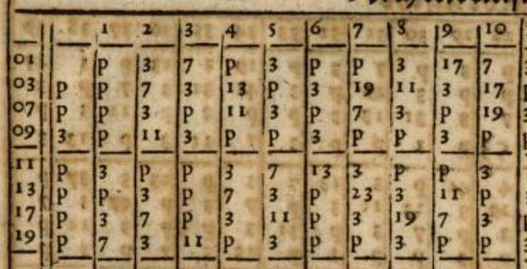
\includegraphics[width=0.6\textwidth]{pic/rahn.jpg}
    \end{center}}

  \onslide<4->{Ejemplo: $611 = 13\cdot 47$ y $613$ es primo.}
\end{frame}

\begin{frame}
  \frametitle{TABLAS DE FACTORIZACIÓN}

  \onslide<2->{Johann Poetius, 1728, tabla de factorizaciones completas para
    $n < 10\,000$ («anatomia numerorum», \emph{anatomía de los números}).}
  % https://www.digitale-sammlungen.de/en/view/bsb10082579
 
  \visible<3->{\begin{center}
      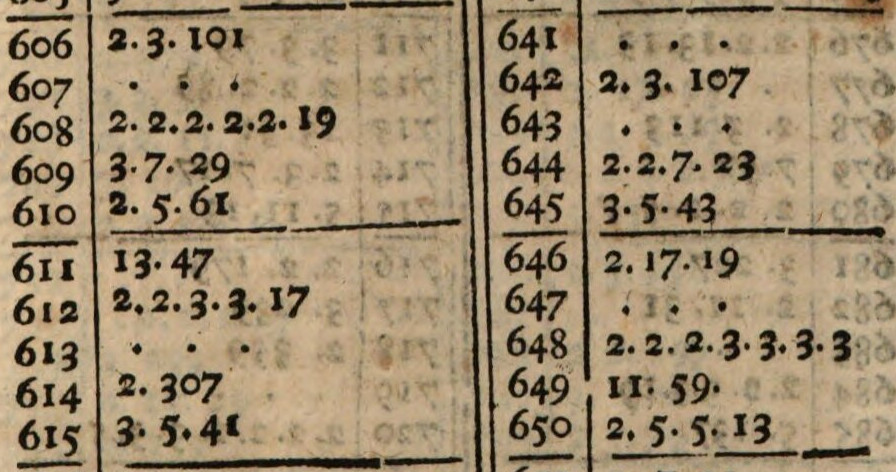
\includegraphics[width=0.8\textwidth]{pic/poetius.jpg}
    \end{center}}
\end{frame}

\begin{frame}
  \frametitle{ENUNCIADOS SIN LA UNICIDAD}

  \onslide<2->{La posibilidad de descomponer todo número en un producto de
      primos se menciona en varios textos del siglo XVIII.}

  \begin{itemize}
  \item<3-> Euler «Vollständige Anleitung zur Algebra» (1770)

    (\emph{Guía completa de álgebra}), Cap. IV, no. 41.

  \item<4-> Legendre, «Essai sur la théorie des nombres» (1798)

    (\emph{Ensayo sobre la teoría de números}), Introduction, \S VIII.
  \end{itemize}
\end{frame}

\begin{frame}
  \frametitle{GAUSS, «DISQUISITIONES» (1801)}

  \onslide<2->{«Disquisitiones arithmeticae», Sectio secunda, no. 16:

    \vspace{1em}

    «Numerus compositus quicunque \underline{unico tantum modo} in factores
    primos resolui potest».

    \vspace{1em}

    (Cualquier número compuesto puede resolverse en factores primos
    \underline{de modo único}.)}
\end{frame}

\begin{frame}[plain,noframenumbering]

  \vfill

  \begin{center}\huge\headingfont
    DEMOSTRACIÓN
  \end{center}

  \vfill
\end{frame}

\begin{frame}
  \frametitle{FACTORIZACIÓN EN PRIMOS}

  \begin{itemize}
  \item<2-> $p > 1$ es \textbf{primo} si
    $d \mid p \Longrightarrow d = \pm 1, \pm p$.

  \item<3-> Para dos primos $p \mid q \Longrightarrow p = q$.

  \item<4-> \textbf{Lema de Euclides}:
    $p \mid ab \Longrightarrow p\mid a \text{ o }p\mid b$.

  \item<5-> Todo $n > 1$ tiene un divisor primo:
    \begin{gather*}
      p = d_i \mid d_{i-1} \mid \cdots \mid d_1 \mid d_0 = n, \\
      d_i < d_{i-1} < \cdots < d_1 < d_0.
    \end{gather*}

  \item<6-> Todo $n > 1$ se descompone en primos:
    $$p_1 \mid n, ~ p_2 \mid \frac{n}{p_1}, ~ p_3 \mid \frac{n}{p_1 p_2}, ~ p_4 \mid \frac{n}{p_1 p_2 p_3}, ~ \ldots, ~ n = p_1 \cdots p_s.$$
  \end{itemize}
\end{frame}

\begin{frame}
  \frametitle{TEOREMA FUNDAMENTAL DE LA ARITMÉTICA}

  \begin{itemize}
  \item<2-> Todo $n \ne 0$ puede ser escrito como
    $$n = \pm p_1 \cdots p_s,$$
    donde los $p_i$ son primos (no necesariamente distintos).

  \item[*]<3-> Si $n = \pm 1$, entonces $s = 0$ (producto vacío).

  \item<4-> Para dos factorizaciones de esta forma
    $$\pm p_1 \cdots p_s = \pm q_1 \cdots q_t$$
    necesariamente $s = t$ y $p_i = q_i$ para $i = 1,\ldots,s$,
    después de una permutación de los índices.
  \end{itemize}
\end{frame}

\begin{frame}
  \frametitle{DEMOSTRACIÓN DE LA UNICIDAD}

  \onslide<2->{\[ p_1 \cdots p_s = q_1 \cdots q_t. \]}

  \begin{itemize}
  \item<3-> \textbf{Lema de Euclides}:
    $p_s \mid q_1 \cdots q_t \Longrightarrow p_s \mid q_i \Longrightarrow p_s = q_i$

    para algún $i = 1,\ldots,t$.

  \item<4-> Después de una renumeración, $i = t$.

  \item<5-> $p_1 \cdots p_{s-1} \cancel{p_s} = q_1 \cdots q_{t-1} \cancel{q_t}$.

  \item<6-> . . . . .

  \item<7-> Llegamos a la conclusión que $s = t$ y $p_i = q_i$ después de una
    permutación de los índices. \qed
  \end{itemize}
\end{frame}

\begin{frame}
  \frametitle{OTRA FORMULACIÓN}

  \begin{itemize}
  \item<2-> Todo entero $n \ne 0$ se escribe de modo único como
    $$n = \pm p_1^{e_1}\cdots p_s^{e_s},$$
    donde $p_1, \ldots, p_s$ son diferentes primos y $e_i \ge 0$.

  \item<3-> Todo número racional $x = \frac{a}{b} \ne 0$ se escribe de modo
    único como
    $$x = \pm p_1^{e_1}\cdots p_s^{e_s},$$
    donde $p_1, \ldots, p_s$ son diferentes primos y $e_i \in \ZZ$.

  \item<4-> La potencia $e_i$ de $p_i$ es la \textbf{valuación $p_i$-ádica} del
    número.

  \item<5-> En otra ocasión: valuaciones $p$-ádicas.
    \onslide<6->{\begin{gather*}
      v_2 (252) = 2, ~
      v_3 (252) = 2, ~
      v_7 (252) = 1, \\
      v_p (252) = 0 \text{ si } p\ne 2,3,7, \quad 257 = 2^2\cdot 3^2\cdot 7.
    \end{gather*}}
    \end{itemize}
\end{frame}

\begin{frame}
  \frametitle{ALGORITMOS}

  \begin{itemize}
  \item<2-> Existen algoritmos rápidos que verifican si $p$ es primo.

    \textbf{Algoritmo probabilista de Miller--Rabin} (1980).

    \textbf{Algoritmo determinista AKS} (Agrawal--Kayal--Saxena, 2002).

  \item<3-> No se conocen (probablemente no existen) algoritmos rápidos de
    factorización en primos. Esta es la base de la
    \textbf{criptografía de clave pública}.

  \item<4-> El mejor algoritmo práctico para grandes números:

    la \textbf{criba del cuerpo de números}
    (Pollard--Lenstra--Lenstra--\dots, 1988).

  \item<5-> El \textbf{algoritmo de Shor} (1994) para las computadoras
    cuánticas. Todavía tiene poco valor práctico.
  \end{itemize}
\end{frame}

\begin{frame}[plain,noframenumbering]

  \vfill

  \begin{center}\huge\headingfont
    ALGUNAS APLICACIONES

    (EJERCICIOS)
  \end{center}

  \vfill
\end{frame}

\begin{frame}
  \frametitle{EJERCICIO 1: REINTERPRETACIÓN\\DEL MCD Y MCM}

  \onslide<2->{\begin{framed}
      Escribamos
      \[
        m = p_1^{e_1}\cdots p_s^{e_s},
        \quad
        n = p_1^{e'_1}\cdots p_s^{e'_s},
      \]
      donde $p_i$ son primos y $e_i, e_i' \ge 0$. Luego,
      \[ m \mid n \iff e_i \le e'_i \text{ para todo }i. \]
      \[
        \mcd (m,n) = \prod_i p_i^{\min \{ e_i, e_i' \}},
        \quad
        \mcm (m,n) = \prod_i p_i^{\max \{ e_i, e_i' \}}.
      \]
    \end{framed}}

  \onslide<3->{\textbf{Demostración}. Ejercicio.}
\end{frame}

\begin{frame}
  \frametitle{REINTERPRETACIÓN DEL MCD Y MCM (CONTINUACIÓN)}

  \begin{itemize}
  \item<2-> \textbf{Ejemplo}:
    \begin{align*}
      \mcd (120, 90) & = \mcd (2^3\cdot 3\cdot 5, \, 2\cdot 3^2\cdot 5) = 30, \\
      \mcm (120, 90) & = 2^3\cdot 3^2\cdot 5 = 360.
    \end{align*}

  \item<3-> mcd y mcm se calculan con el algoritmo de Euclides que es muy
    rápido, mientras que la factorización es difícil.

  \item<4-> Nuestra prueba del teorema fundamental usa el mcd:

    $\text{existencia del mcd} \Longrightarrow
    \text{lema de Euclides} \Longrightarrow
    \text{teorema fundamental}$.
  \end{itemize}
\end{frame}

\begin{frame}
  \frametitle{EJERCICIO 2: DIVISIBILIDAD POR NÚMEROS COPRIMOS}

  \begin{itemize}
  \item<2-> Demuestre que si $\mcd (a,b) = 1$, entonces
    $$a \mid c, \, b \mid c \Longrightarrow ab \mid c.$$

  \item<3-> Demuestre que para todo $n$ se tiene
    \[
      30 \mid (n^5 - n),
      \quad
      42 \mid (n^7 - n).
    \]

    \onslide<4->{Ejemplo:
    \begin{align*}
      2^2 - 2 & = 30,\\
      3^2 - 3 & = 240 = 30\cdot 8,\\
      4^2 - 4 & = 1020 = 30\cdot 34,\\
      5^2 - 5 & = 3120 = 30\cdot 104,\\
              & \cdots
    \end{align*}}
  \end{itemize}
\end{frame}

\begin{frame}
  \frametitle{EJERCICIO 3: N-ÉSIMAS POTENCIAS}

  \begin{itemize}
  \item<2-> Demuestre que $n = p_1^{e_1}\cdots p_s^{e_s}$ es un cuadrado
    ($n = m^2$ para algún $m$) si y solamente si los $e_i$'s son pares.

  \item<3-> Demuestre que si $a^2 = bc$ y $\mcd (b,c) = 1$, entonces
    $b = b'^2$ y $c = c'^2$ para algunos $b', c' \in \ZZ$.

  \item<4-> Generalice estas observaciones a $n$-ésimas potencias.
  \end{itemize}
\end{frame}

\begin{frame}
  \frametitle{EJERCICIO 4: FUNCIÓN DE MÖBIUS μ}

  \begin{itemize}
  \item<2-> Si $p^2 \mid n$ para algún $p$, entonces $\mu (n) \dfn 0$.

  \item<3-> Si $n = p_1\cdots p_s$ para diferentes primos $p_i$, entonces
    $\mu (p_1\cdots p_s) \dfn (-1)^s$.

  \item<4-> Demuestre que
    $\sum_{d\mid n} \mu (d) = 0$,
    donde la suma es sobre los divisores positivos de $n$.

    \onslide<5->{Ejemplo:
    \begin{multline*}
      \mu(1) + \mu(2) + \mu(3) + \mu(4) + \mu(6) + \mu(9) + \mu(12) + \mu(18) + \mu(36) \\
      = 1 - 1 - 1 + 0 + 1 + 0 + 0 + 0 + 0 = 0.
    \end{multline*}}

  \item<6-> En otra ocasión: \textbf{inversión de Möbius}.
  \end{itemize}
\end{frame}

\begin{frame}[plain,noframenumbering]

  \vfill

  \begin{center}\huge\headingfont
    ¡GRACIAS POR SU ATENCIÓN!
  \end{center}

  \vfill
\end{frame}
\end{document}


% \input{valuaciones-p-adicas.tex}
% \input{funciones-multiplicativas-e-inversion-de-moebius.tex}
% \input{ternas-pitagoricas-y-descenso.tex}
% \input{distribucion-de-primos.tex}

% \part{Aritmética módulo n}

% \input{motivacion-ecuaciones-diofanticas.tex}
% \input{congruencias-y-residuos-mod-n.tex}
% \input{teorema-chino-del-residuo.tex}
% \input{residuos-invertibles-y-funcion-de-euler.tex}
% \input{teorema-de-lagrange.tex}
% \input{raices-primitivas.tex}
% \input{teorema-de-dos-cuadrados.tex}
% \input{lema-de-hensel.tex}
% \input{principio-local-global.tex}

% \part{Reciprocidad cuadrática}

% \input{simbolo-de-legendre.tex}
% \input{reciprocidad-cuadratica.tex}
% \input{simbolo-de-jacobi.tex}

% \appendix
% \input{lista-de-primos.tex}

% \backmatter

% \cleardoublepage

% \phantomsection

% \addcontentsline{toc}{chapter}{Bibliografía}

% \bibliography{tn-intro}
% \bibliographystyle{amsalpha-cust}

\end{document}
